\chapter{Fondamenta Teoriche}
Gran parte dell'intelligenza artificiale moderna si fonda sull'utilizzo del
\textbf{Deep Learning} \cite{lecun2015DeepLearning}, grazie alla sua capacità
intrinseca di estrarre le \textit{features} dai dati, superando i limiti del
\textit{Machine Learning} tradizionale. Ad oggi, il DL viene utilizzato in una
grande varietà di domini, come l'elaborazione del linguaggio naturale, oppure
la visione artificiale, o ancora la robotica. Tuttavia, le reti neurali
\textit{feed-forward} presentano una grave limitazione, ovvero l'assenza di uno
stato interno, che non ne permette l'utilizzo con dati in sequenza, come i
video, gli audio o il testo. Al fine di ovviare a questa mancanza, sono state
introdotte le \textbf{Reti Neurali Ricorrenti}, specificatamente pensate per
l'elaborazione di dati sequenziali di qualsiasi tipologia.
\begin{figure}[H]
    \centering
    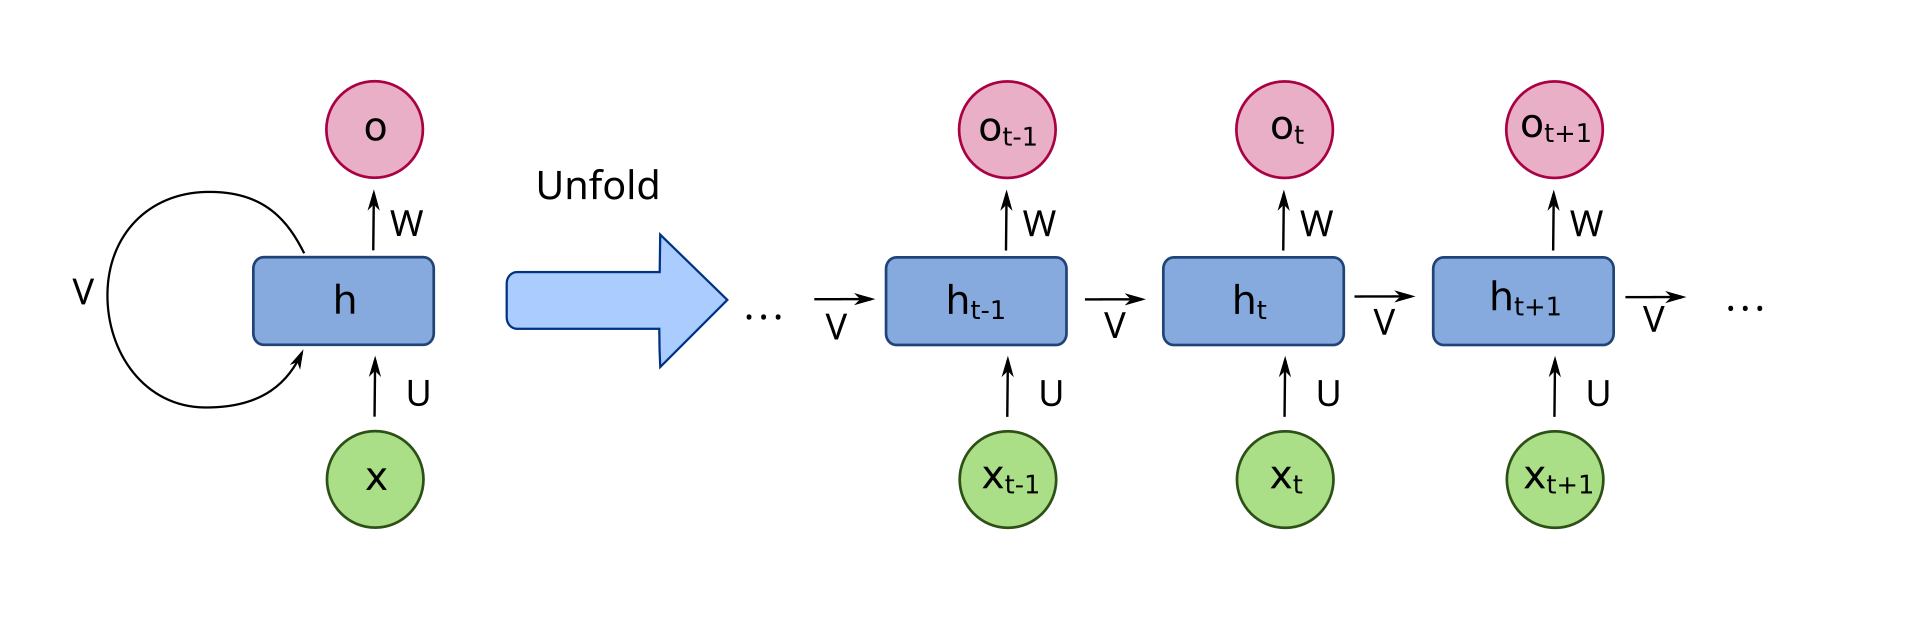
\includegraphics[width=0.8\textwidth]{images/SOTA/rnn.png}
    \caption{Rete Neurale Ricorrente e \textit{unfolding}. Fonte: \url{https://commons.wikimedia.org/w/index.php?curid=60109157} }
\end{figure}
Nonostante la capacità teorica delle RNN di processare sequenze di lunghezza arbitraria, la loro applicazione pratica è limitata a causa di una serie di problematiche molto note. Come dimostrato matematicamente da Bengio et al. \cite{bengio1994learning}, l'addestramento di questi modelli è ostacolato dal fenomeno della scomparsa o dell'esplosione del gradiente. Questa criticità rende estremamente difficile per il modello correlare informazioni distanti all'interno della sequenza temporale. Al fine di contrastare questi fenomeni nascono le reti \textbf{Long Short Term Memory} (LSTM) \cite{lstm} e \textbf{Gated Recurrent Units} (GRU) \cite{DBLP:journals/corr/ChoMGBSB14}, che introducono il concetto di \textit{gating} per contrastare le problematiche legate al gradiente. Per anni questa tipologia di modelli ha costituito lo stato dell'arte per i dati sequenziali, nonostante delle limitazioni note, ad esempio la necessità di elaborare i dati in modo sequenziale (parola per parola nel caso di elaborazione del linguaggio naturale) rendendo impossibile la parallelizzazione del calcolo tramite hardware moderno (GPU), oppure la difficoltà con le dipendenze a lungo termine all'interno delle sequenze.
\section{I modelli Transformer}
I modelli \textit{Transformer} trovano le loro origini nel meccanismo di
\textbf{Attenzione}, nato anni prima nell'ambito dei modelli
\textit{encoder-decoder}, in particolare con le reti \textit{seq2seq}
\cite{seq2seq}, utilizzate nell'ambito della traduzione automatica. In questa
tipologia di modelli il \textit{decoder}, tipicamente costituito da una RNN,
utilizza un unico vettore, lo stato finale dell'\textit{encoder} (anche in
questo caso si trattava solitamente di una RNN), che riassume la sequenza di
input per poi generare l'output.
\begin{figure}[H]
    \centering
    \includegraphics[width=0.7\textwidth]{images/SOTA/seq2seq.png}
    \caption{Inferenza con modelli \textit{seq2seq}. Fonte: \url{https://github.com/d2l-ai/d2l-en} }
\end{figure}
La grande limitazione di questi modelli risiede proprio nell'utilizzo di un singolo vettore statico per la fase di decodifica, che non risulta sufficiente a riassumere adeguatamente la sequenza in input. Inoltre, se quest'ultima risulta particolarmente lunga, dato l'utilizzo di modelli RNN o LSTM, le informazioni legate ai primi dati in ingresso potevano essere perdute a causa della grande distanza dallo stato finale. Allo scopo di superare i limiti del vettore di contesto e migliorare quindi le prestazioni dei modelli \textit{seq2seq} viene introdotto per la prima volta un meccanismo di attenzione da Bahdanau et al. \cite{bahdanau2016neuralmachinetranslationjointly}.
\begin{figure}[H]
    \centering
    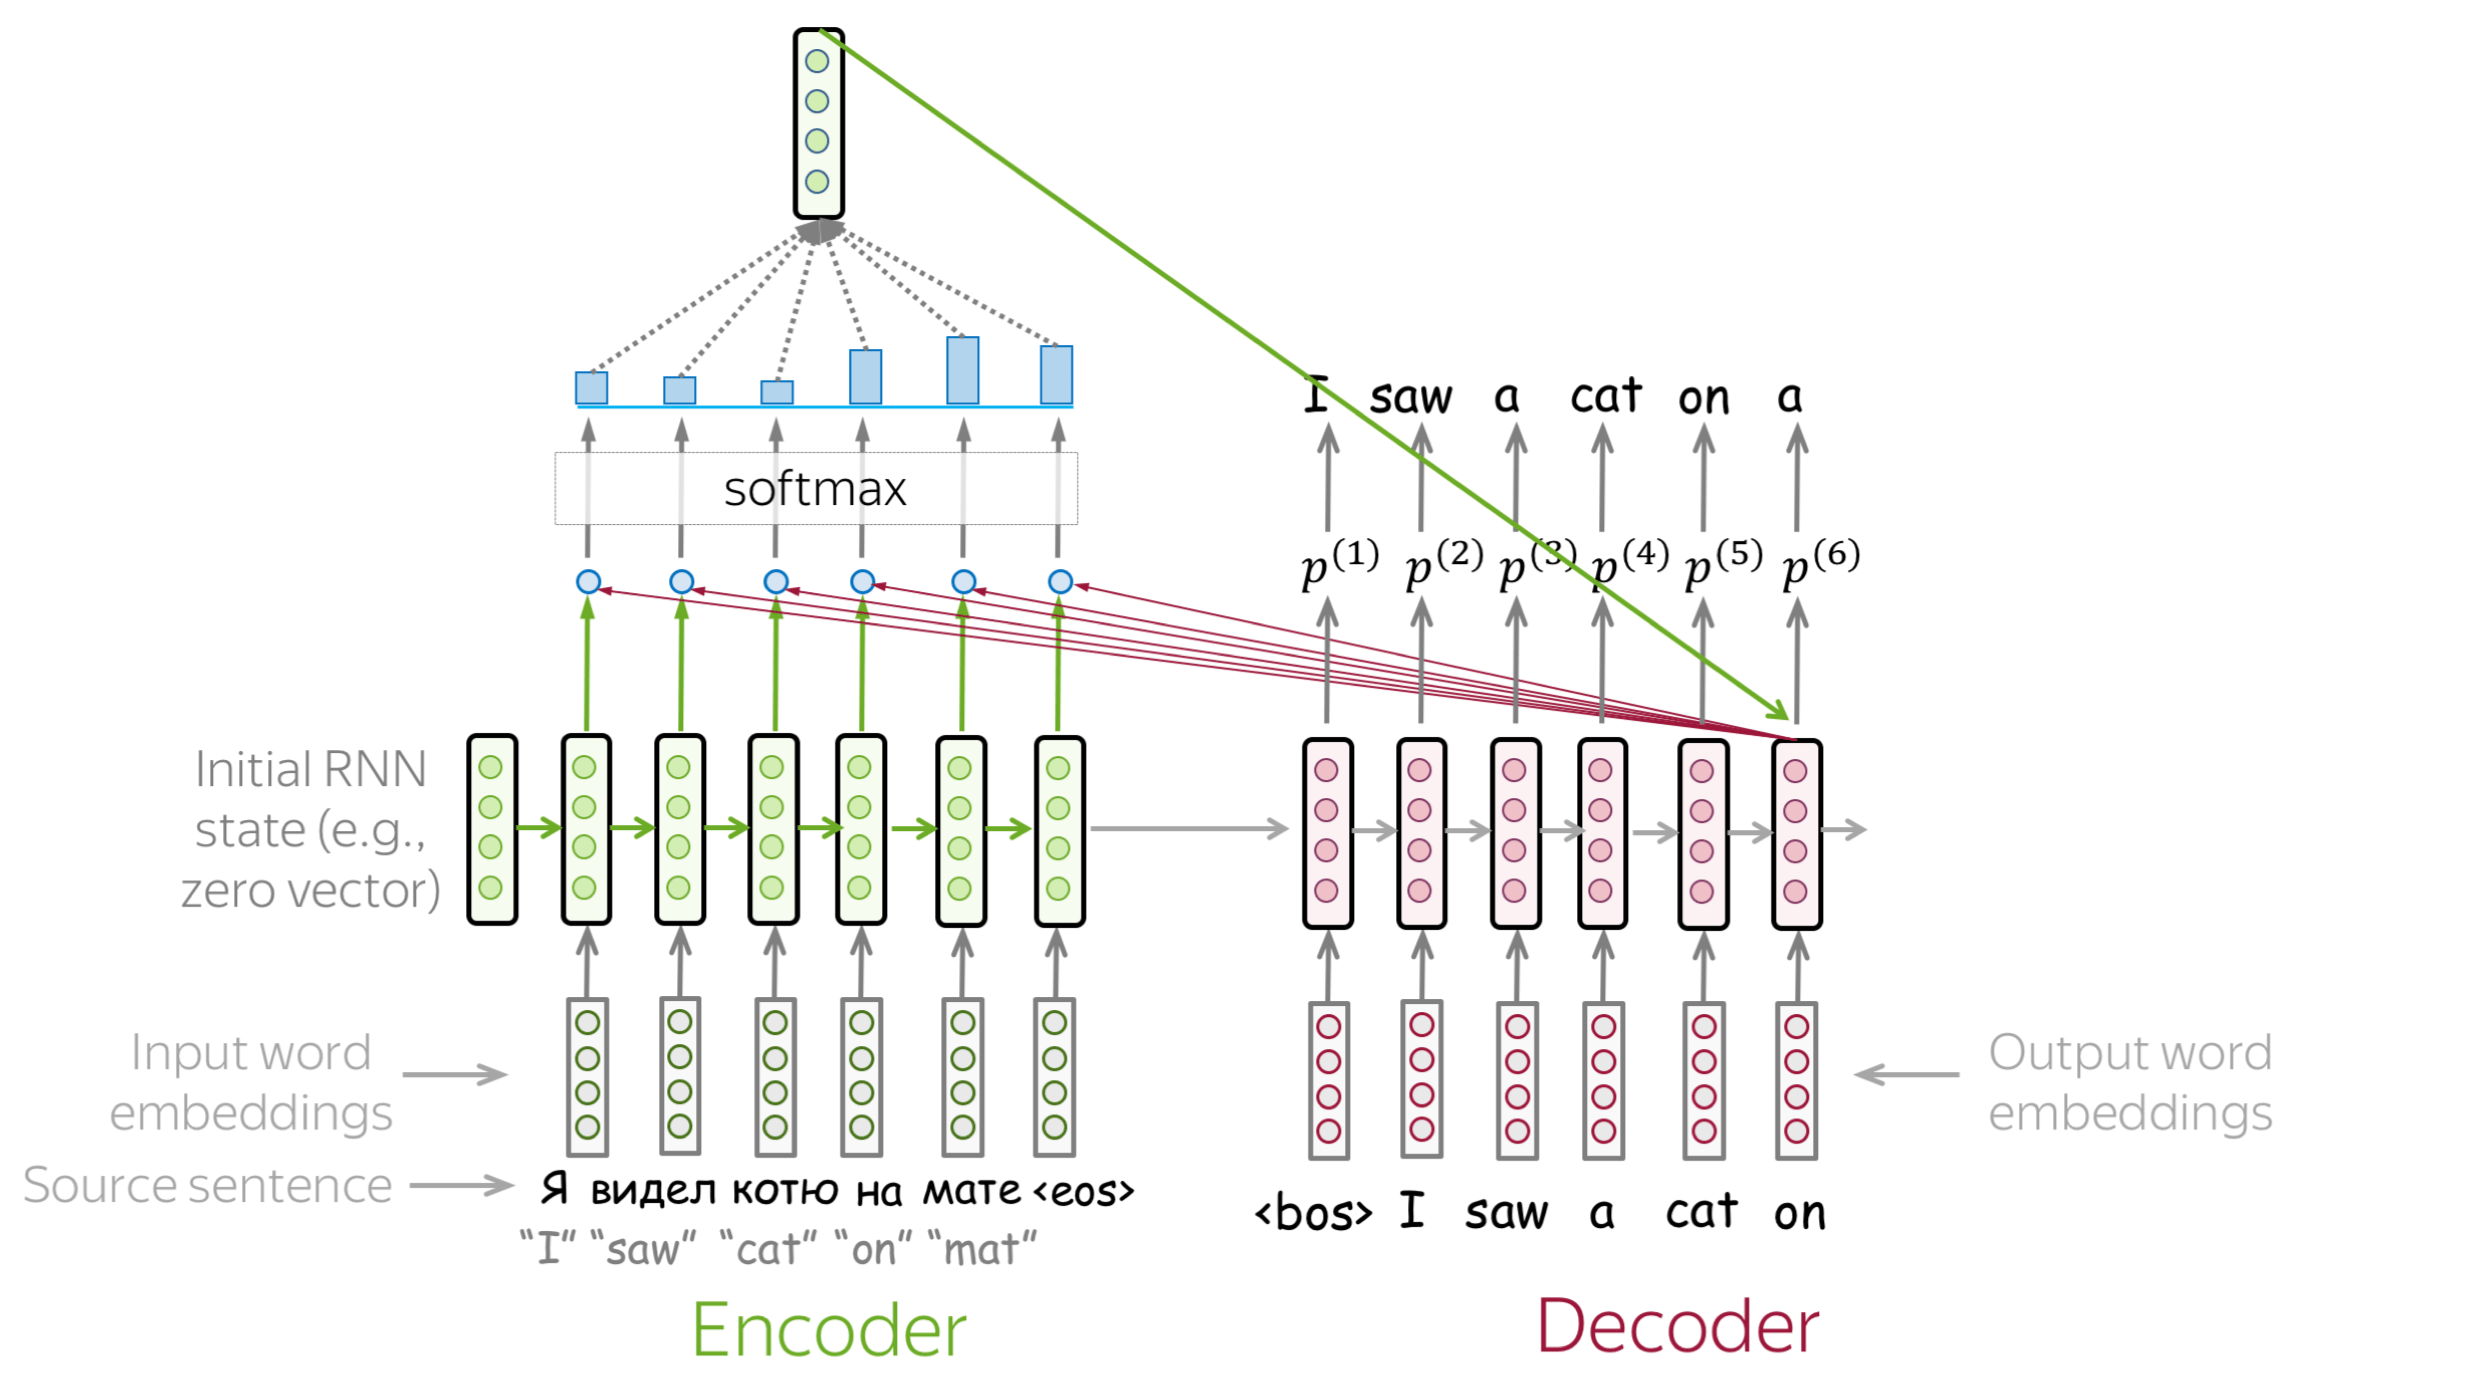
\includegraphics[width=1.0\textwidth]{images/SOTA/attn.png}
    \caption{Meccanismo di attenzione nei modelli \textit{seq2seq}. Fonte: \url{https://lena-voita.github.io/nlp_course/seq2seq_and_attention.html} }
\end{figure}
Questo meccanismo rende dinamico il vettore di contesto, che viene calcolato per ogni iterazione di decodifica pesando i contributi di tutti gli stati intermedi ottenuti dall'\textit{encoder}. In questo modo è possibile fornire in input al modello \textit{decoder} un vettore che riassume adeguatamente la sequenza in ingresso, dando maggiore importanza alle porzioni realmente rilevanti per l'output e migliorando nettamente le prestazioni dei modelli \textit{seq2seq}. \par
Nonostante l'introduzione dell'attenzione abbia rappresentato una svolta nel
superamento del limite costituito dal vettore di contesto statico, queste
architetture rimanevano ancora profondamente legate alla natura sequenziale
delle RNN o LSTM. In tale configurazione, l'attenzione agisce solo come un
meccanismo ausiliario tra l'\textit{encoder} e il \textit{decoder}, e
l'elaborazione dei dati avviene un passo alla volta, impedendo qualsiasi tipo
di parallelizzazione dei calcoli. \par
La vera rivoluzione si verifica con l'introduzione dell'architettura
\textbf{Transformer} \cite{AttentionIsAllYouNeed}, che abbandona interamente
l'approccio sequenziale delle reti ricorrenti per passare a quello delle reti
\textit{feed-forward}, utilizzando la \textbf{Multi-Head Self Attention}. In
particolare, l'architettura proposta da Vaswani et al. è di tipo
\textit{encoder-decoder}, poiché è stata utilizzata e testata sul dominio della
traduzione automatica.
\begin{figure}[H]
    \centering
    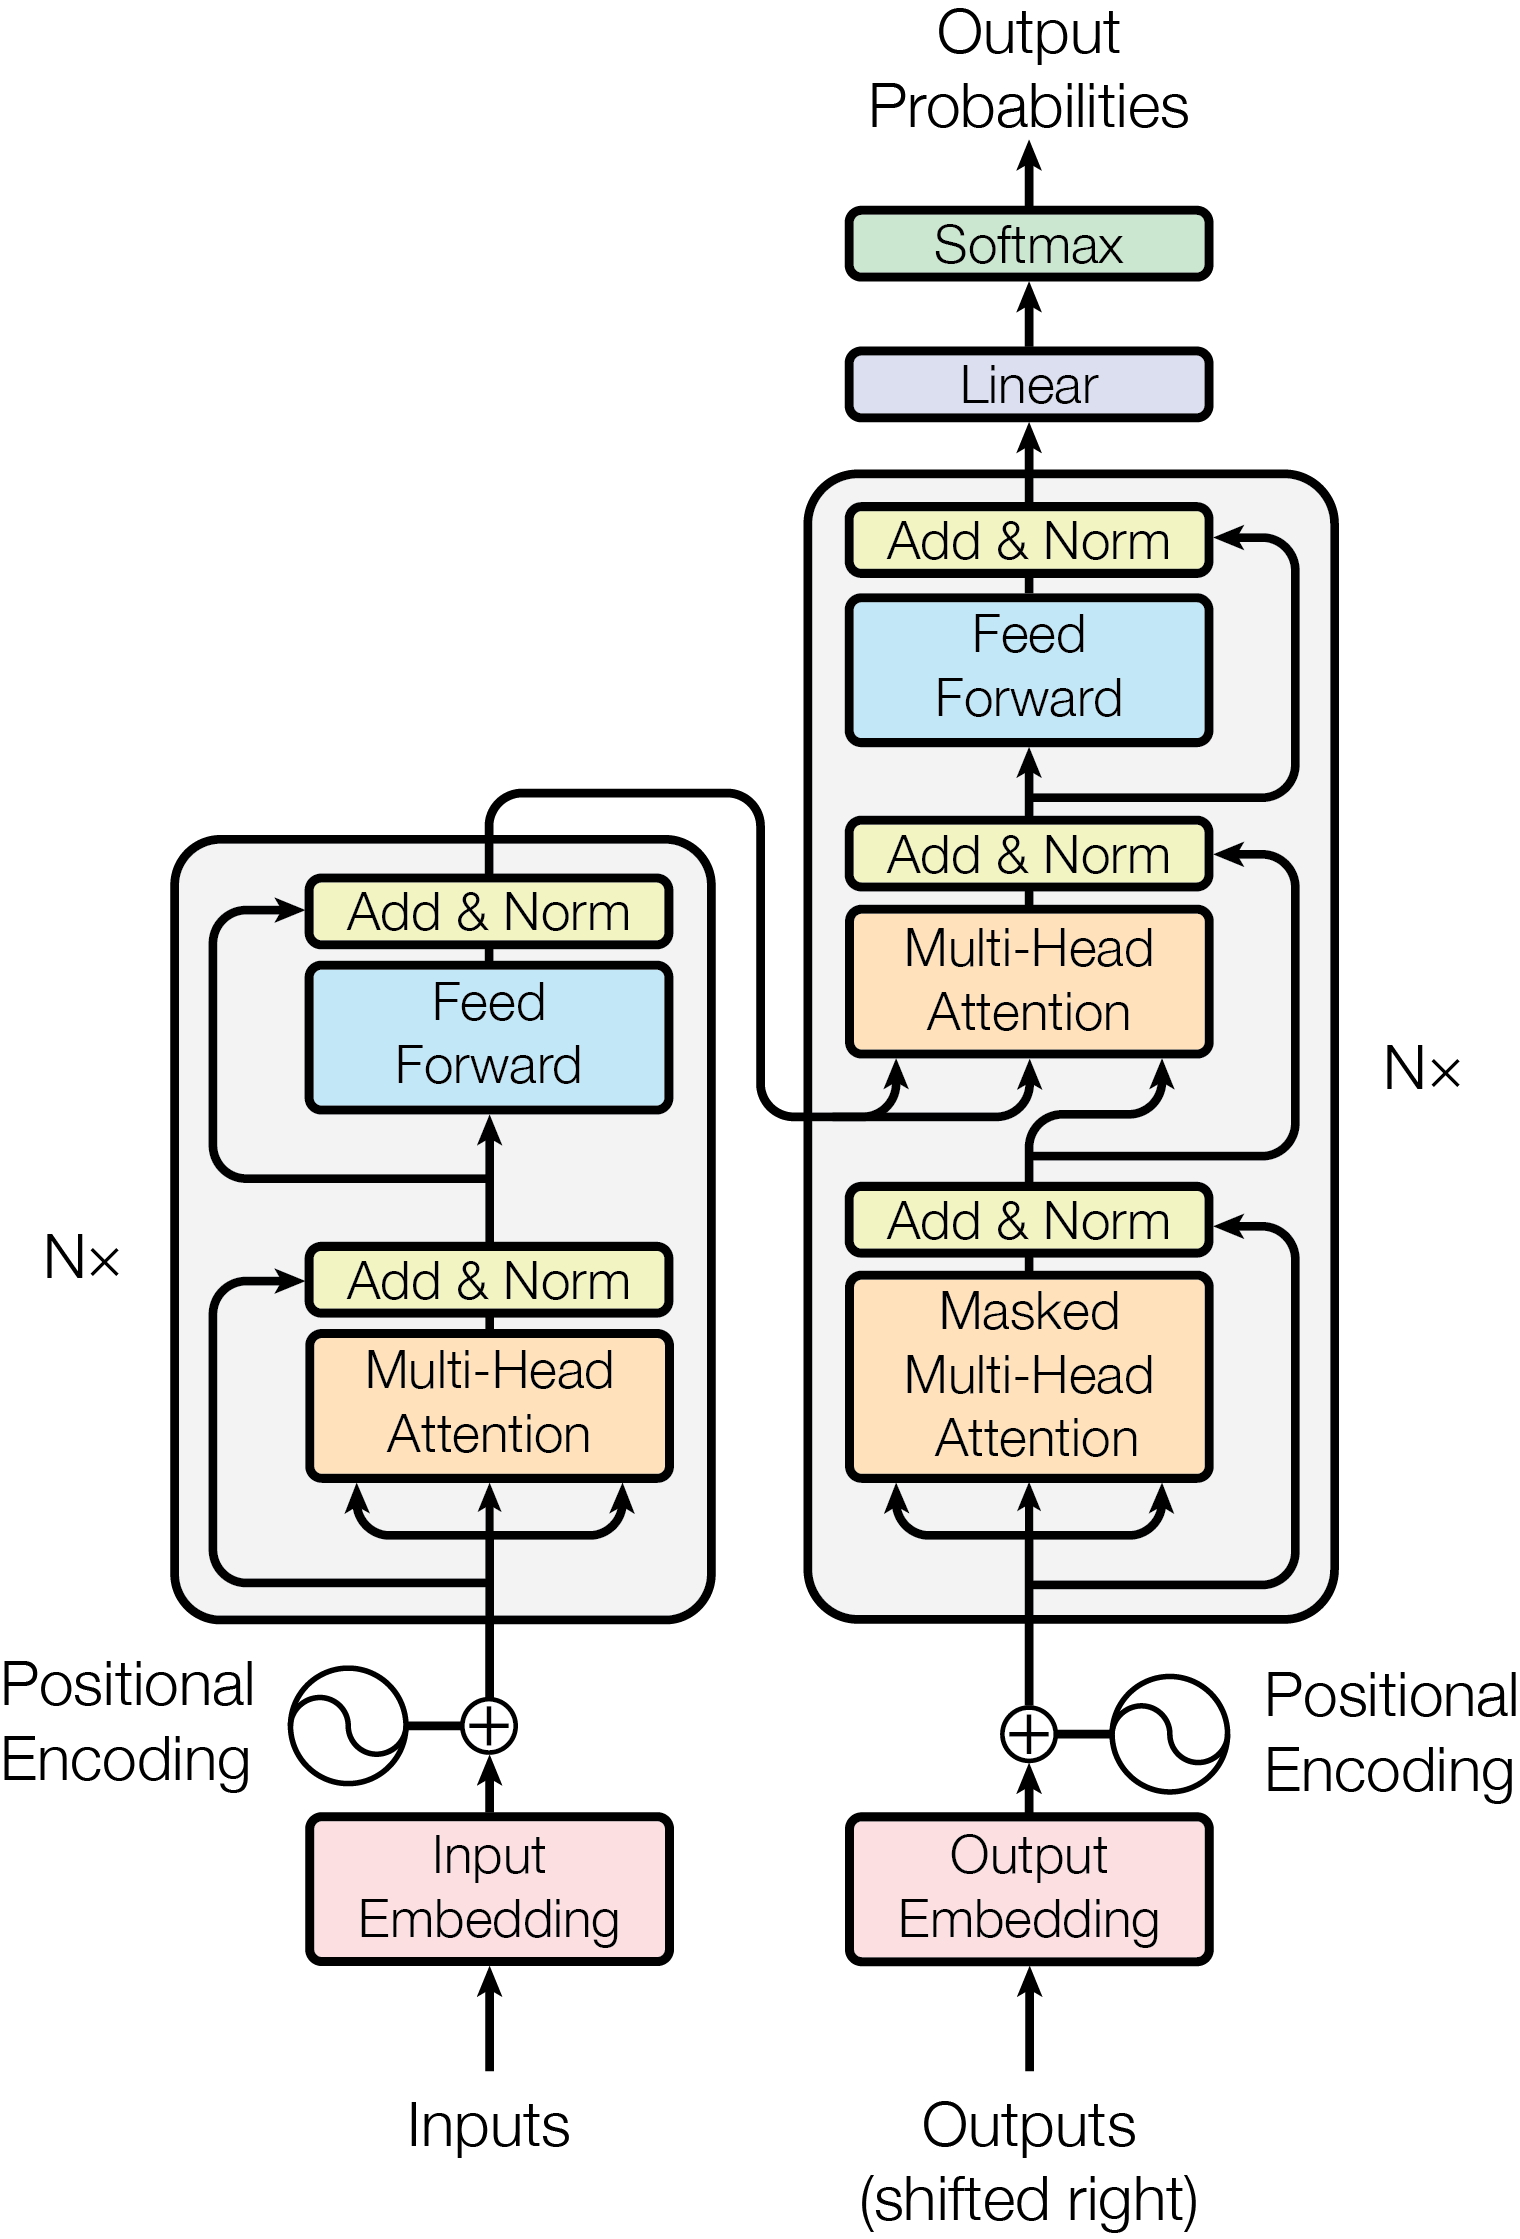
\includegraphics[width=0.5\textwidth]{images/SOTA/Transformer.png}
    \caption{Architettura Transformer originaria proposta da Vaswani et al. Fonte: \cite{AttentionIsAllYouNeed} }
    \label{figure:attn_is_all_you_need}
\end{figure}
Questa architettura si compone di una serie di blocchi, i cosiddetti blocchi \textit{Transformer}, posti in cascata attraverso un flusso residuale (al fine di evitare i fenomeni della scomparsa dei gradienti) e formati da tra componenti principali:
\begin{itemize}
    \item \textbf{Multi-Head Self Attention (MHSA):} rappresenta il cuore del blocco, permette al modello di proiettare l'input in diversi spazi di rappresentazione e catturare relazioni globali tra gli elementi della sequenza.

    \item \textbf{Layer Normalization (LayerNorm):} introdotta da Ba et al. \cite{ba2016layernormalization}, viene applicata prima (o dopo, a seconda della variante \textit{Pre-Norm} o \textit{Post-Norm} \cite{xiong2020layernormalizationtransformerarchitecture}) di ogni blocco funzionale, stabilizza le attivazioni e accelera la convergenza dell'addestramento, garantendo che la distribuzione dei dati rimanga consistente attraverso i vari layer.

    \item \textbf{Feed-Forward Network (FFN):} tipicamente costituita da due trasformazioni lineari intervallate da una funzione di attivazione non lineare (come la \textit{GELU} \cite{hendrycks2023gaussianerrorlinearunits} o la \textit{ReLU} \cite{agarap2019deeplearningusingrectified}). Questo modulo, spesso chiamato \textbf{MLP} (\textit{Multi-Layer Perceptron}), opera in modo indipendente su ogni posizione della sequenza, permettendo di elaborare e ricombinare le informazioni estratte dal meccanismo di attenzione.
\end{itemize}
Notare che l'architettura Transformer non possiede meccanismi intrinseci per gestire l'ordine sequenziale dei dati (a differenza delle RNN), di conseguenza è necessario introdurre il \textbf{Positional Encoding}(\cite{shaw2018selfattentionrelativepositionrepresentations}\cite{su2023roformerenhancedtransformerrotary}). Si tratta di vettori che vengono sommati ai vettori di input per fornire al modello informazioni sulla posizione relativa o assoluta di ogni elemento nella sequenza.
Il nodo cruciale di questa architettura è il meccanismo di \textbf{Self Attention}, che risulta strutturalmente differente da quanto introdotto da Bahdanau et al. \cite{bahdanau2016neuralmachinetranslationjointly}, poiché non si tratta più di un calcolo di similarità tra lo stato corrente del \textit{decoder} (output) e gli stati intermedi dell'\textit{encoder} (input). In questo nuovo meccanismo sono i singoli elementi della sequenza in input che interagiscono tra di loro, permettendo di catturare le dipendenze contestuali indipendentemente dalla distanza fra gli elementi coinvolti. In particolare, la \textit{Self Attention}, detto $x$ un elemento della sequenza in input $X = {x_1, x_2,\dots, x_n}$, esegue tre proiezioni lineari che producono le \textit{query}, le \textit{key} e i \textit{value}
\begin{equation}
    \begin{aligned}
        q & = W_q x \\
        k & = W_k x \\
        v & = W_v x
    \end{aligned}
\end{equation}
Considerato l'i-esimo elemento della sequenza $x_i$, viene calcolato il prodotto scalare tra la \textit{query} corrispondente $q_i$ e le \textit{key} di tutti gli altri elementi della sequenza. Il risultato esprime il grado di affinità o "attenzione" che l'elemento i-esimo deve porre verso gli altri elementi. Questi punteggi vengono poi normalizzati ad una distribuzione di probabilità tramite una funzione \textit{softmax}.
\begin{equation}
    \alpha_{ij} = \text{softmax} \left( \frac{q_i \cdot k_j}{\sqrt{d_k}} \right) = \frac{\exp \left( \frac{q_i \cdot k_j}{\sqrt{d_k}} \right)}{\sum_{l=1}^{n} \exp \left( \frac{q_i \cdot k_l}{\sqrt{d_k}} \right)}
\end{equation}
Infine, viene eseguita una somma pesata dei vettori \textit{value} $v$ per ottenere l'uscita del meccanismo di attenzione.
\begin{equation}
    a_i = \sum_{j=1}^{n} \alpha_{ij} v_j
\end{equation}
Tuttavia, il vero punto di forza dell'architettura Transformer risiede nella capacità di parallelizzare questa operazione attraverso la \textbf{Scaled-Dot-Product Attention}.
\begin{figure}[H]
    \centering
    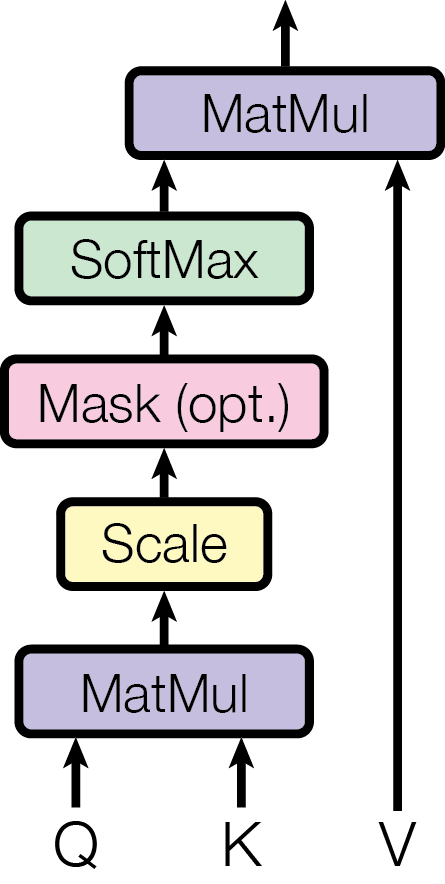
\includegraphics[width=0.2\textwidth]{images/SOTA/mhsa_detail.png}
    \caption{Visualizzazione dell'operazione di \textit{Scaled-Dot-Product Attention}. Fonte: \cite{AttentionIsAllYouNeed} }
    \label{figure:attn_mask}
\end{figure}
Invece di calcolare l'attenzione un elemento alla volta, le proiezioni di tutti gli $n$ elementi della sequenza vengono raggruppate in matrici $Q, K, V \in \mathbb{R}^{n \times d}$, permettendo di eseguire l'intero calcolo tramite il prodotto matriciale, facilmente parallelizzabile tramite hardware apposito (GPU oppure TPU).
\begin{equation}
    \text{Attention}(Q, K, V) = \text{softmax} \left( \frac{QK^T}{\sqrt{d_k}} \right) V
\end{equation}
Questa formulazione evidenzia i costi computazionali dell'architettura: il prodotto $QK^T$ genera una matrice di attenzione di dimensione $n \times n$, portando a una complessità quadratica $O(n^2)$ (temporale e spaziale) rispetto alla lunghezza della sequenza. Di conseguenza, il vantaggio rispetto alle architetture RNN, dato dalla possibilità di parallelizzare e velocizzare le operazioni sull'intera sequenza, comporta un aumento del costo computazionale (le RNN hanno costo lineare $O(n)$). \par
Al fine di aumentare la capacità di questa nuova architettura viene introdotto
il concetto di \textbf{Multi-Head Attention}, attraverso il quale è possibile
dotare il meccanismo di attenzione di molteplici "teste" che operano estraendo
\textit{features} e rappresentazioni differenti dalla sequenza in input. Quanto
descritto in precedenza viene applicato all'interno di ogni \textit{attention
    head} e successivamente gli output vengono concatenati e proiettati in uno
spazio della dimensione originale della rappresentazione.
\begin{figure}[H]
    \centering
    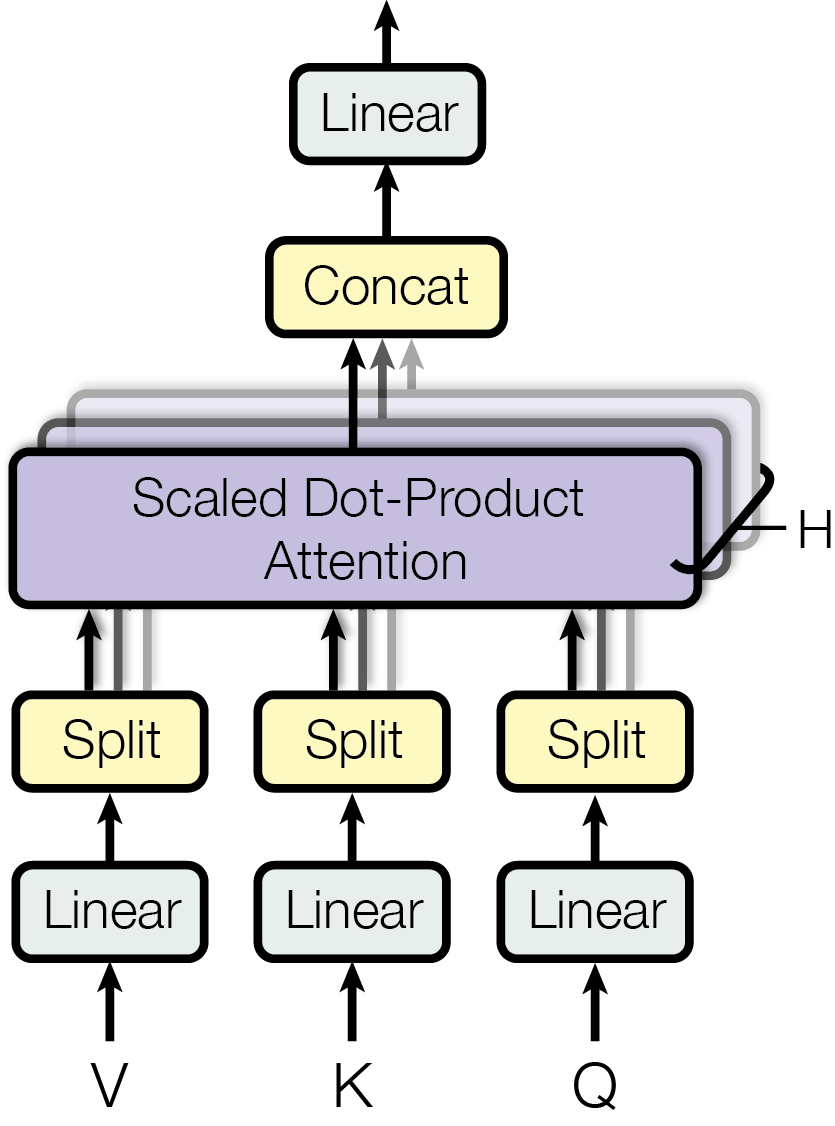
\includegraphics[width=0.35\textwidth]{images/SOTA/MHSA.png}
    \caption{\textit{Multi Head Self Attention}. Fonte: \cite{AttentionIsAllYouNeed} }
\end{figure}

Per concludere la trattazione dei modelli \textit{transformer} è necessario affrontare
l'utilizzo della \textbf{mascheratura} (\textit{masking}). Come è possibile
notare dalla Figura \ref{figure:attn_is_all_you_need}, vi sono due tipologie di
blocchi \textit{Transfomer}: i blocchi \textit{encoder} e i blocchi
\textit{decoder}. Nei primi, ogni elemento può interagire con ogni altro
elemento della sequenza (attenzione bi-direzionale), permettendo di estrarre
una rappresentazione contestuale completa di contesto destro e sinistro. Al
contrario, nei secondi (usati nei modelli generativi di linguaggio), viene
applicata una maschera durante la fase di attenzione (Figura
\ref{figure:attn_mask}). Tale maschera pone a $-\infty$ i valori della matrice
di attenzione relativi agli elementi successivi nella sequenza, garantendo che,
attraverso la funzione \textit{softmax}, i pesi di attenzione corrispondenti
vengano azzerati. In questo modo la predizione (della parola successiva, nel
caso dei modelli generativi del linguaggio) dipenderà esclusivamente dai
termini che la precedono (contesto sinistro), preservando così la causalità
necessaria durante l'inferenza.
\section{Vision Transformer}
Per quanto concerne l'ambito della visione artificiale, per anni le \textbf{Reti Neurali Convoluzionali} (CNN) hanno dominato il campo grazie alla loro capacità di estrarre le \textit{features} spaziali delle immagini attraverso l'uso di filtri appresi che vengono applicati alle immagini. Il successo delle CNN è dovuto principalmente a due proprietà intrinseche: l'\textbf{invarianza alla traslazione} e la \textbf{località dei dati}. Grazie ai filtri convoluzionali, queste reti sono in grado di riconoscere pattern indipendentemente dalla loro posizione nell'immagine e di elaborare le relazioni tra pixel vicini in modo estremamente efficiente. Tuttavia, questo approccio presenta un limite fondamentale: la natura locale delle convoluzioni rende difficile catturare le \textbf{relazioni a lungo raggio} tra pixel distanti, se non attraverso l'utilizzo di numerosi strati, posti in cascata, che aumentano progressivamente il campo ricettivo (\textit{receptive field}) \cite{luo2017understandingeffectivereceptivefield}. \par
\begin{figure}[H]
    \centering
    \includegraphics[width=0.8\textwidth]{images/SOTA/ViT_original.pdf}
    \caption{Architettura del Vision Transformer (ViT). Fonte: \cite{dosovitskiy2021imageworth16x16words} }
\end{figure}
L'introduzione dei modelli \textit{Transformer} ha portato alla nascita dei \textbf{Vision Transformer} (ViT) \cite{dosovitskiy2021imageworth16x16words}, che utilizzano un'architettura \textit{Encoder-Only} per applicare il meccanismo di attenzione all'ambito della visione artificiale. In particolare, l'architettura ViT suddivide l'immagine in regioni, dette \textit{patch}, non sovrapposte (ad esempio, \textit{patch} di dimensione $16 \times 16$ pixel), che vengono poi appiattiti e proiettati in uno spazio di rappresentazione tramite una trasformazione lineare. Questi vettori di rappresentazione delle patch vengono quindi arricchiti con informazioni posizionali e forniti ad una serie di blocchi \textit{Transformer-Encoder} simili a quelli descritti in precedenza. \par
\begin{figure}[H]
    \centering
    
\includegraphics[width=0.8\textwidth]{images/MHSA.png}
    \caption{Struttura della \textit{Multi Head Attention}.}
\end{figure}
\begin{figure}[H]
    \centering
    \includegraphics[width=0.8\textwidth]{images/MLP.png}
    \caption{Struttura del \textit{Multi Layer Perceptron} nei blocchi Transformer del ViT.}
\end{figure}
Sfruttando il meccanismo di attenzione, i ViT permettono alle regioni dell'immagine di interagire tra loro, catturando relazioni a lungo raggio molto più facilmente rispetto alle CNN. Nonostante i ViT abbiano dimostrato prestazioni competitive rispetto alle CNN, soprattutto su dataset di grandi dimensioni, presentano ancora alcune limitazioni, come la necessità di grandi quantità di dati per l'addestramento \cite{steiner2022trainvitdataaugmentation} e la complessità computazionale elevata, dovuta alla natura quadratica del meccanismo di attenzione. Tuttavia, l'utilizzo di questi modelli sta crescendo rapidamente (soprattutto come \textit{backbone} o \textit{Vision Encoder} all'interno di architetture modulari \cite{kirillov2023segment}\cite{radford2021learningtransferablevisualmodels}), portando a numerose varianti e miglioramenti che cercano di mitigare queste criticità, come l'introduzione di meccanismi di attenzione più efficienti o l'adozione di approcci ibridi che combinano le CNN con i ViT. \par
\begin{figure}[H]
    \centering
    \includegraphics[width=0.4\textwidth]{images/SOTA/DeiT.pdf}
    \caption{Architettura del Data-efficient Image Transformer (DeiT). Fonte: \cite{touvron2021trainingdataefficientimagetransformers}}
\end{figure}
Una delle prime varianti che hanno migliorato il ViT originale è stata il \textbf{Data-efficient Image Transformer} (DeiT) \cite{touvron2021trainingdataefficientimagetransformers}, che ha introdotto un nuovo metodo di addestramento chiamato \textit{knowledge distillation}, in cui un modello ("student") viene addestrato a imitare le predizioni di un modello pre-addestrato ("teacher"), ottenendo prestazioni competitive anche con dataset di dimensioni ridotte. Questa tecnica, applicata ad uno speciale \textit{token} di distillazione, ha permesso al DeiT di raggiungere risultati paragonabili a quelli del ViT originale, ma con un minor quantitativo di dati.
\begin{figure}[H]
    \centering
    \includegraphics[width=1.0\textwidth]{images/SOTA/SWIN_arch.pdf}
    \caption{Architettura di \textit{Swin Transformer}. Fonte: \cite{liu2021swintransformerhierarchicalvision}}
\end{figure}
Successivamente, è stato proposto lo \textbf{Swin Transformer} \cite{liu2021swintransformerhierarchicalvision}, che introduce meccanismi di attenzione gerarchici e a finestre mobili per migliorare l'efficienza computazionale. A differenza del ViT che mantiene una risoluzione costante, lo \textit{Swin Transformer} riduce gradualmente la risoluzione spaziale man mano che si scende in profondità nella rete, unendo le patch vicine (Patch Merging). Questo crea una struttura gerarchica simile a quella delle reti neurali convoluzionali (CNN), permettendo al modello di vedere sia dettagli piccoli che strutture grandi. Inoltre, invece di calcolare l'attenzione su tutta l'immagine, lo \textit{Swin Transformer} la calcola all'interno di finestre locali di \textit{patch} non sovrapposte, introducendo meccanismi di località simili a quelli delle CNN.
\begin{figure}[H]
    \centering
    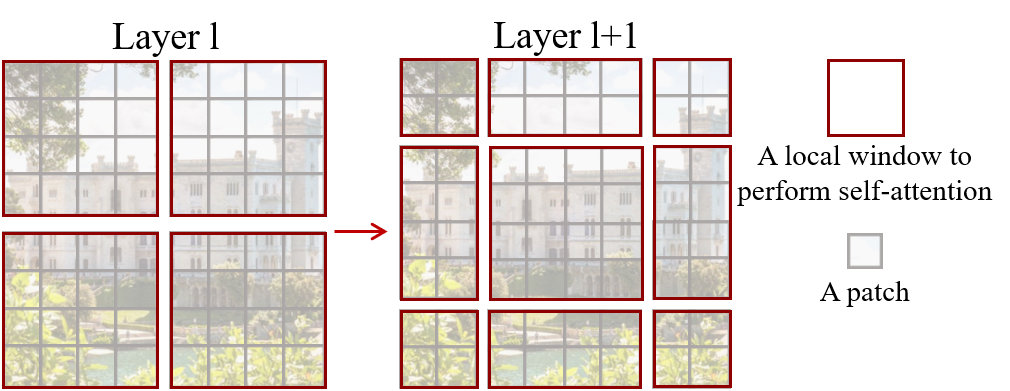
\includegraphics[width=0.7\textwidth]{images/SOTA/SWIN_window.png}
    \caption{Meccaniscmo di Shifted Window. Fonte: \cite{liu2021swintransformerhierarchicalvision}}
\end{figure}
Allo stesso tempo viene introdotto un meccanismo di \textit{Shifted Window} che permette alle finestre di patch di interagire tra loro nel blocco successivo, garantendo che le informazioni vengano propagate attraverso l'intera immagine. Grazie a queste innovazioni, lo \textit{Swin Transformer} è in grado di raggiungere prestazioni all'avanguardia su una varietà di compiti di visione artificiale, come la classificazione delle immagini, il rilevamento degli oggetti e la segmentazione semantica, con un'efficienza computazionale significativamente migliorata rispetto al ViT originale. \par
